\chapter{CholecInstanceSeg: Tool Instance Segmentation for Laparoscopic Surgery}
\chaptermark{CholecInstanceSeg}
\label{chap:cholecinstanceseg}
\minitoc

\begin{center}
\begin{minipage}[b]{0.9\linewidth}
\small
\textbf{Chapter note.}
This chapter adapts material from the Scientific Data paper \emph{CholecInstanceSeg: A Tool Instance Segmentation Dataset for Laparoscopic Surgery}. The chapter is written as the dataset foundation for the subsequent work on grounded surgical action triplets.
\end{minipage}
\end{center}

\section{Overview}
\label{sec:cholecinstanceseg-overview}

The previous chapters motivate surgical scene understanding as a central problem in computer-assisted intervention. A recurring limitation in this area is that many datasets describe the presence of tools or provide semantic tool regions, but do not distinguish between individual tool instances. This distinction matters in laparoscopic surgery because multiple instruments of the same class may appear in the same frame and may participate in different actions. A model that only knows that a grasper is present cannot reliably determine which grasper is retracting tissue, which one is idle, or which one is interacting with a particular anatomical target.

This chapter presents CholecInstanceSeg, a large-scale dataset for surgical tool instance segmentation in laparoscopic cholecystectomy. The dataset contains 41,933 annotated frames from 85 clinical procedures and 64,483 tool instances. Each visible surgical instrument is annotated with a semantic class and an instance identifier, enabling pixel-level localisation and separation of individual tools. The annotated classes are grasper, bipolar, hook, clipper, scissors, irrigator, and snare.

The role of this chapter in the thesis is twofold. First, it establishes a high-quality data resource for instrument instance segmentation in routine human laparoscopic surgery. Second, it provides the spatial representation needed by \Chapref{chap:triplet-grounding}, where instrument instances are linked to surgical action triplets.

\section{Motivation}
\label{sec:cholecinstanceseg-motivation}

Minimally invasive surgery relies on indirect vision through a laparoscope or endoscope. This creates a constrained and visually challenging operating environment, with a limited field of view, frequent occlusion, smoke, specular reflection, motion blur, dirty lenses, and visually similar tool shafts. Computer-assisted intervention systems must therefore interpret scenes from image evidence that is often ambiguous and incomplete.

Tool localisation is one of the most basic requirements for such systems. It supports downstream tasks including workflow analysis, tool-tissue interaction recognition, surgical skill assessment, camera control, and context-aware assistance. However, many public surgical tool datasets are limited in one or more ways: they focus on porcine or ex-vivo settings, contain a small number of annotations, provide only semantic segmentation, or offer instance information for only a restricted set of tool classes. These limitations restrict the development of models that need to reason about individual instrument instances.

\begin{table}[ht]
\centering
\resizebox{\linewidth}{!}{
\begin{tabular}{|l|l|l|l|l|l|l|}
\hline
\textbf{Dataset} & \textbf{Patient} & \textbf{Environment} & \textbf{Procedures} & \textbf{Annotations} & \textbf{Semantic} & \textbf{Instance} \\
\hline
Endovis2015 \cite{bodenstedt2018comparative} & Human & Ex-vivo/In-vivo & 8 & 10k & 3 classes & No \\
\hline
Endovis2017 \cite{endovis2017} & Porcine & In-vivo & 10 & 2.4k & 10 classes & No \\
\hline
Endovis2018 \cite{endovis2018} & Porcine & In-vivo & 16 & 2.4k & 10 classes & No \\
\hline
CholecSeg8k \cite{cholecseg8k} & Human & In-vivo & 17 & 8k & 12 classes & No \\
\hline
AutoLaparo \cite{autolaparo} & Human & In-vivo & 21 & 1.8k & 7 classes & No \\
\hline
ROBUSTMIS2019 \cite{robustmis2019} & Human & In-vivo & 30 & 10k & 2 classes & Yes \\
\hline
SAR-RARP50 \cite{psychogyios2023sar} & Human & In-vivo & 50 & 10k & 10 classes & No \\
\hline
CholecInstanceSeg & Human & In-vivo & 85 & 41.9k & 8 classes & Yes \\
\hline
\end{tabular}}
\caption{Comparison of representative datasets used in surgical tool segmentation research. CholecInstanceSeg provides instance-level annotations at a larger scale than the listed alternatives while focusing on routine human laparoscopic cholecystectomy.}
\label{tab:cholecinstanceseg-dataset-comparison}
\end{table}

CholecInstanceSeg was designed to address this gap by expanding existing cholecystectomy datasets with instance segmentation labels. The resulting resource is not only useful for training instance segmentation models, but also for integrating tool localisation with other annotations derived from the same parent videos, such as phase labels, action triplets, and critical view of safety assessment.

\section{Data Sources}
\label{sec:cholecinstanceseg-data-sources}

CholecInstanceSeg was created from frames extracted from three public laparoscopic cholecystectomy datasets: Cholec80 \cite{EndoNet}, CholecT50 \cite{NWOYE2022102433_rendevous}, and CholecSeg8k \cite{cholecseg8k}. These datasets are public subsets of the CAMMA Cholec120 collection \cite{twinanda2018rsdnet}. Their relationship is shown in \figref{fig:cholecinstanceseg-source-relationships}.

\begin{figure}[ht]
\centering
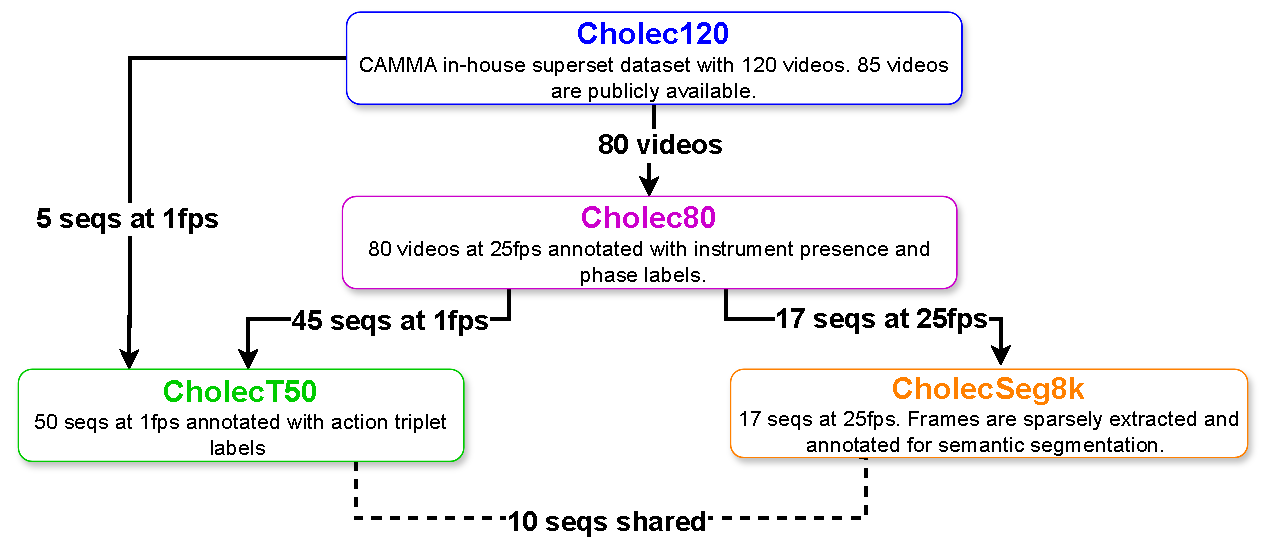
\includegraphics[width=\linewidth]{figs/cholecinstanceseg/cholec_dataset_relationships.pdf}
\caption{Relationship between the source datasets used to construct CholecInstanceSeg. Cholec80, CholecT50, and CholecSeg8k are public subsets of the larger Cholec120 collection. Some image sequences are shared between CholecT50 and CholecSeg8k, although their frame extraction protocols differ.}
\label{fig:cholecinstanceseg-source-relationships}
\end{figure}

Cholec80 contains 80 cholecystectomy videos with phase and tool-presence labels. CholecT50 contains 50 image sequences annotated with instrument-action-target triplets. CholecSeg8k contains 8,080 frames with semantic segmentation labels. The overlap between these resources makes them valuable for building multi-annotation surgical datasets, but it also requires careful accounting of shared sequences, frame extraction rates, and potential redundancy across partitions.

The frames from Cholec80 and CholecT50 are primarily at 854 by 480 pixels, with three CholecT50 sequences available at 1920 by 1080 pixels. CholecT50 provides pre-extracted image sequences at 1 frame per second. For Cholec80 videos not covered by CholecT50 or CholecSeg8k, frames were extracted at a sparse rate of one frame every 30 seconds of the original 25 fps video stream, with additional frames included when a sequence would otherwise contain fewer than 50 sampled frames.

\section{Dataset Construction}
\label{sec:cholecinstanceseg-construction}

The final dataset is organised into four partitions, shown in \figref{fig:cholecinstanceseg-map}. These partitions balance annotation density and procedure diversity.

\begin{figure}[ht]
\centering
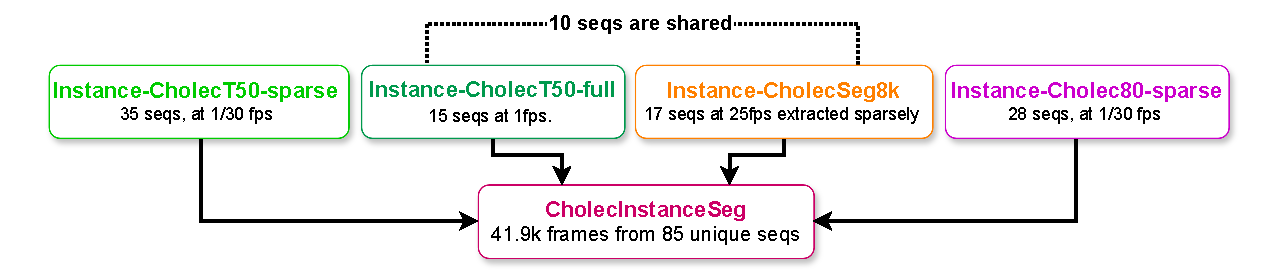
\includegraphics[width=\linewidth]{figs/cholecinstanceseg/cholec_instance_seg_map.pdf}
\caption{Composition of CholecInstanceSeg. The dataset combines dense and sparse partitions from CholecT50, CholecSeg8k, and Cholec80. The mixed strategy provides dense supervision for selected sequences while preserving broad coverage across procedures.}
\label{fig:cholecinstanceseg-map}
\end{figure}

\begin{table}[ht]
\centering
\resizebox{\linewidth}{!}{
\begin{tabular}{|l|c|c|c|c|c|}
\hline
 & \textbf{Inst-CholecSeg8k} & \textbf{Inst-CholecT50-sparse} & \textbf{Inst-CholecT50-full} & \textbf{Inst-Cholec80-sparse} & \textbf{Total} \\
\hline
Sequences & 17 (10 shared) & 35 & 15 (10 shared) & 28 & 85 \\
\hline
Frames & 8,080 & 2,681 & 28,317 & 2,855 & 41,933 \\
\hline
Tool instances & 10,523 & 4,098 & 45,221 & 4,641 & 64,483 \\
\hline
\end{tabular}}
\caption{Summary of the CholecInstanceSeg partitions.}
\label{tab:cholecinstanceseg-partitions}
\end{table}

The Instance-CholecSeg8k partition contains all 8,080 frames from CholecSeg8k. Since CholecSeg8k already provided semantic segmentation, this partition served as a useful starting point, but it required conversion to instance segmentation and further correction. The Instance-CholecT50-full partition contains all frames from 15 selected CholecT50 sequences, giving dense supervision for a subset of procedures. The remaining 35 CholecT50 sequences were sampled sparsely to form Instance-CholecT50-sparse. Finally, 28 Cholec80 videos not included in CholecT50 or CholecSeg8k were sampled sparsely to increase procedural diversity.

This mixed design reflects a practical trade-off. Dense instance segmentation of every frame in every sequence would be prohibitively expensive. At the same time, relying only on sparse annotation would limit temporal and scene coverage. CholecInstanceSeg therefore combines dense annotation where it is most useful with sparse annotation across a wider set of procedures.

\section{Annotation Protocol}
\label{sec:cholecinstanceseg-annotation}

The annotation protocol was designed to support consistent instance-level labelling of laparoscopic instruments. The seven annotated tool categories were:

\begin{itemize}
\item grasper,
\item bipolar,
\item hook,
\item clipper,
\item scissors,
\item irrigator,
\item snare.
\end{itemize}

The snare category was included in addition to the six standard Cholec80/CholecT50 tool categories because it has distinct visual characteristics and a distinct surgical function. Objects such as detached clips, sutures, needles, specimen bags, gauze, and camera ports were excluded. Instrument ports were not annotated when no instrument extended from them; when an instrument visibly extended from a port, the visible port segment was annotated as part of the instrument, following the convention used in CholecSeg8k.

The most important annotation principle was to capture every visible instrument instance while preserving the functional shape of the tool, especially the end-effector. Pixel-perfect outlines are unrealistic at this scale, particularly in difficult frames, but the annotations were required to preserve the identity and spatial extent of each instrument. Holes within tools were treated as part of the tool mask, following common conventions in surgical instrument segmentation datasets.

Routine surgical video contains many hard cases. CholecInstanceSeg explicitly accounts for motion blur, smoke, occlusion by tissue or blood, tissue attached to instruments, instruments near the image edge, instruments far from the camera, specular reflection, low lighting, saturated lighting, dirty lenses, camera-port views, and instruments submerged in fluid. Examples of these challenges are shown in \figref{fig:cholecinstanceseg-hard-cases}.

\begin{figure}[ht]
\centering
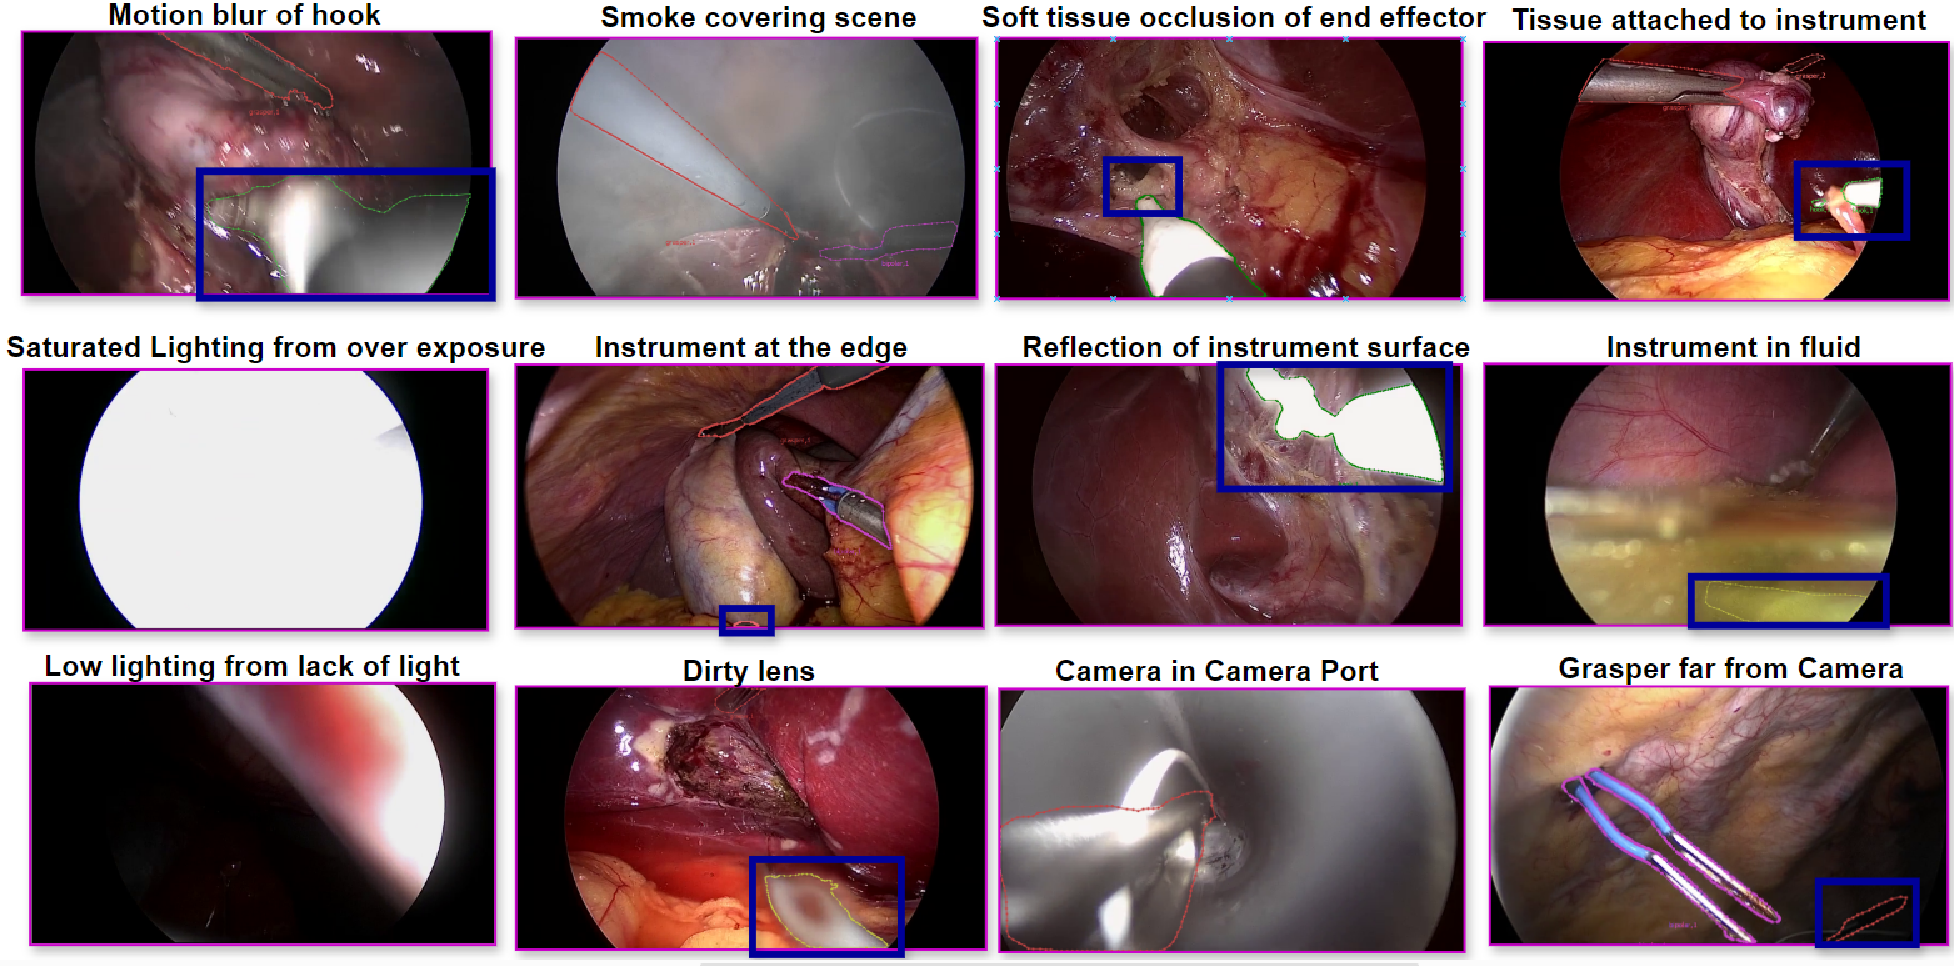
\includegraphics[width=\linewidth]{figs/cholecinstanceseg/all_hard_cases.pdf}
\caption{Examples of challenging annotation cases in CholecInstanceSeg, including motion blur, smoke, soft-tissue occlusion, tissue attachment, lighting artefacts, reflections, dirty lenses, fluid, and edge-of-frame instruments.}
\label{fig:cholecinstanceseg-hard-cases}
\end{figure}

\section{Annotation Tools and Workflow}
\label{sec:cholecinstanceseg-workflow}

Annotation was performed using a lightly customised version of the Segment Anything Annotator tool \cite{wangsupplementary}, built on LabelMe \cite{wada2016labelme} and the Segment Anything Model (SAM) \cite{kirillov2023segment}. The tool was customised to improve navigation, reduce label-file size, and support quality-control workflows. Point-prompt interaction with SAM was used when possible, while manual polygon correction was used in cases where interactive segmentation failed because of smoke, blur, reflection, low contrast, or visually similar background.

For CholecSeg8k, the existing semantic masks were converted into instance masks using class-aware connected components. This approach separates disconnected instruments of the same class and naturally separates instruments of different classes. However, it can fail when the same instrument is split by occlusion, when two instruments of the same class overlap, or when the source semantic mask contains noise. A total of 892 frames with such issues were identified and corrected.

The dense CholecT50-full partition was created with a human-in-the-loop semi-automatic pipeline, shown in \figref{fig:cholecinstanceseg-annotation-pipeline}. Initial annotations from Instance-CholecSeg8k and Instance-CholecT50-sparse were used to train an RTMDet-Ins-l model \cite{lyu2022rtmdet}. The model generated annotation proposals for unlabelled frames, human annotators corrected the proposals, and the corrected labels were then used to retrain the model. This cycle allowed the dataset to scale while retaining human oversight.

\begin{figure}[ht]
\centering
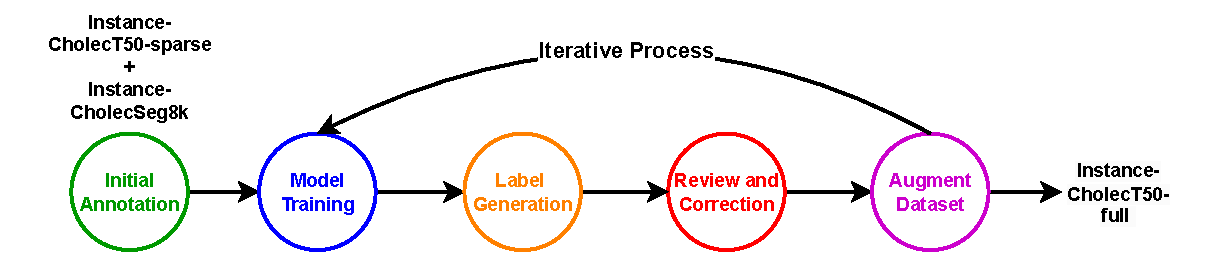
\includegraphics[width=0.9\linewidth]{figs/cholecinstanceseg/train-retrain-annotate.pdf}
\caption{Human-in-the-loop semi-automatic annotation pipeline used for CholecInstanceSeg. Model-generated proposals were reviewed and corrected by annotators, then used to expand the training data for subsequent annotation rounds.}
\label{fig:cholecinstanceseg-annotation-pipeline}
\end{figure}

The overall workflow proceeded in stages: conversion of CholecSeg8k to instance labels, development of the labelling protocol, annotation of the sparse CholecT50 partition, semi-automatic annotation of the dense CholecT50 partition, sparse annotation of additional Cholec80 videos, and final quality control. The primary annotator performed most annotation and quality-control work; a secondary annotator with medical experience supported review, and an expert team mediated ambiguous cases.

\section{Data Records and Splits}
\label{sec:cholecinstanceseg-records}

Annotations follow the LabelMe JSON format. Each annotated shape contains a class label, polygon points, and a group identifier corresponding to the instance ID. When an instrument is represented by multiple polygons, the polygons share a group identifier so that they are treated as a single instance. \Figref{fig:cholecinstanceseg-file-format} summarises the released folder structure and annotation format.

\begin{figure}[ht]
\centering
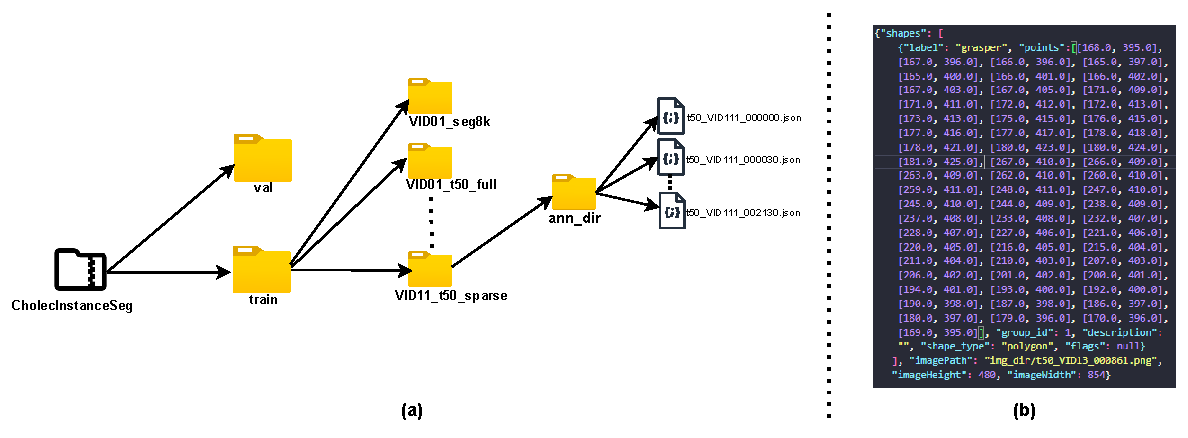
\includegraphics[width=\linewidth]{figs/cholecinstanceseg/file_folder_structure_and_annotation_format.pdf}
\caption{Dataset directory structure and JSON annotation format for CholecInstanceSeg. The format follows LabelMe conventions, with class labels, polygon coordinates, and group identifiers used to recover instrument instances.}
\label{fig:cholecinstanceseg-file-format}
\end{figure}

The recommended split contains 55 training sequences, 17 validation sequences, and 23 test sequences. These splits were designed to account for shared sequences across source datasets, to avoid redundancy between validation/test sets, and to preserve diversity across the evaluation data. The split contains 26,830 training frames, 4,284 validation frames, and 10,819 test frames.

\begin{figure}[ht]
\centering
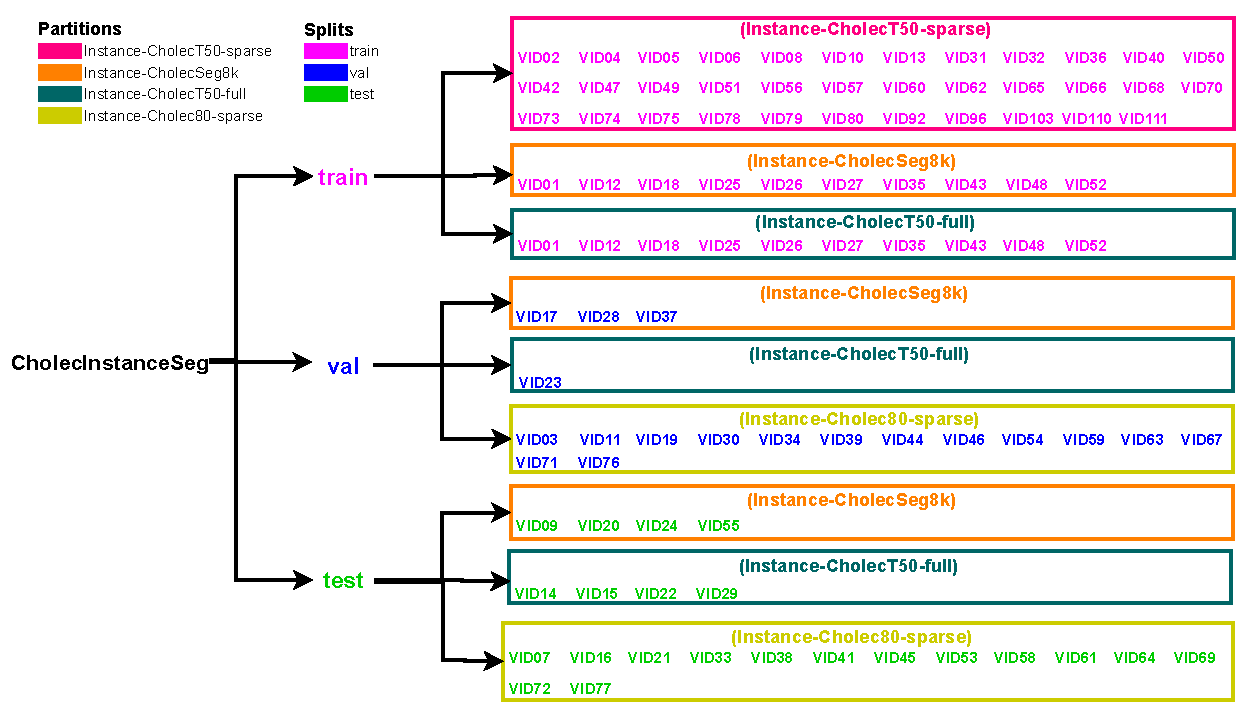
\includegraphics[width=\linewidth]{figs/cholecinstanceseg/train_test_split_dataset_partitions.pdf}
\caption{Recommended training, validation, and test splits for CholecInstanceSeg, accounting for dataset partitions and shared sequences.}
\label{fig:cholecinstanceseg-splits}
\end{figure}

\section{Dataset Analysis}
\label{sec:cholecinstanceseg-analysis}

The class distribution in CholecInstanceSeg is imbalanced, reflecting the realities of laparoscopic cholecystectomy. Graspers are the most frequent instruments, followed by hooks. Irrigators, clippers, scissors, bipolars, and snares occur less often. The number of tools per frame is also uneven: most frames contain one or two visible instruments, with a maximum of four tools in a single frame. Approximately 5,328 frames contain no visible tools.

\begin{figure}[ht]
\centering
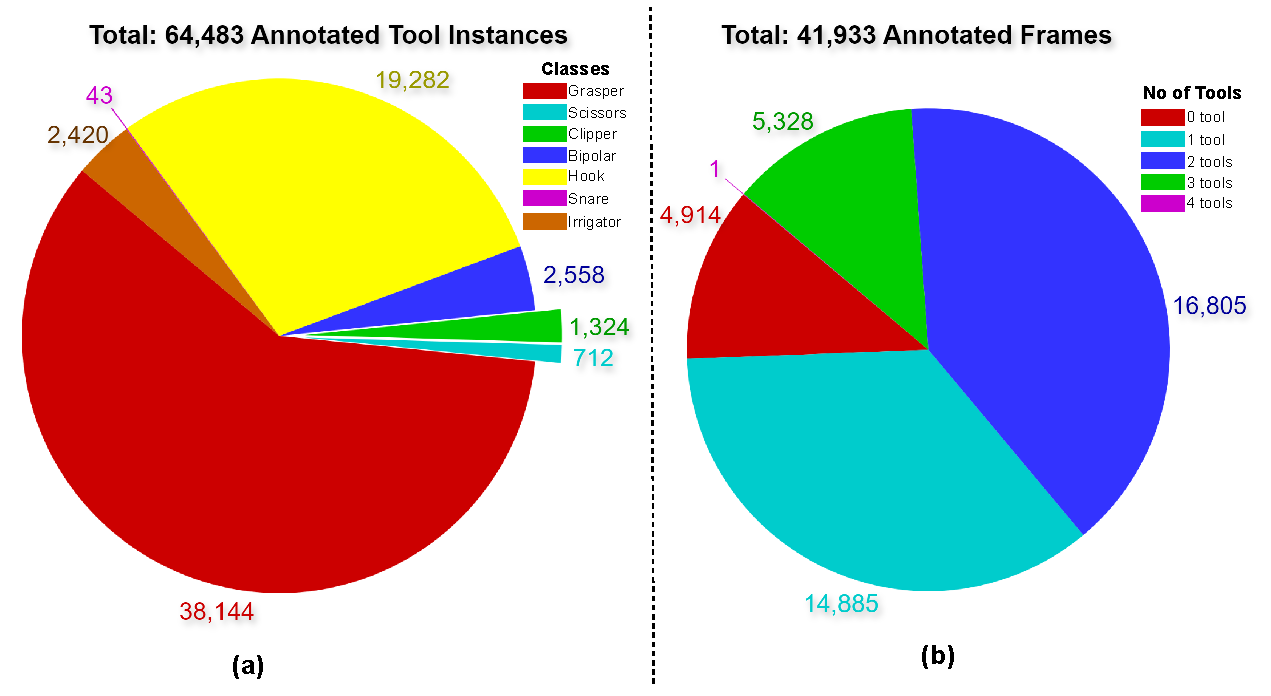
\includegraphics[width=\linewidth]{figs/cholecinstanceseg/charts_instances_spread_and_class_spread.pdf}
\caption{Tool class distribution and number of tool instances per frame in CholecInstanceSeg.}
\label{fig:cholecinstanceseg-class-spread}
\end{figure}

\Figref{fig:cholecinstanceseg-sequence-spread} shows how tool instances are distributed across sequences and partitions. The dense CholecT50-full partition contains the largest number of instances, while the sparse partitions provide additional diversity with fewer frames per sequence.

\begin{figure}[ht]
\centering
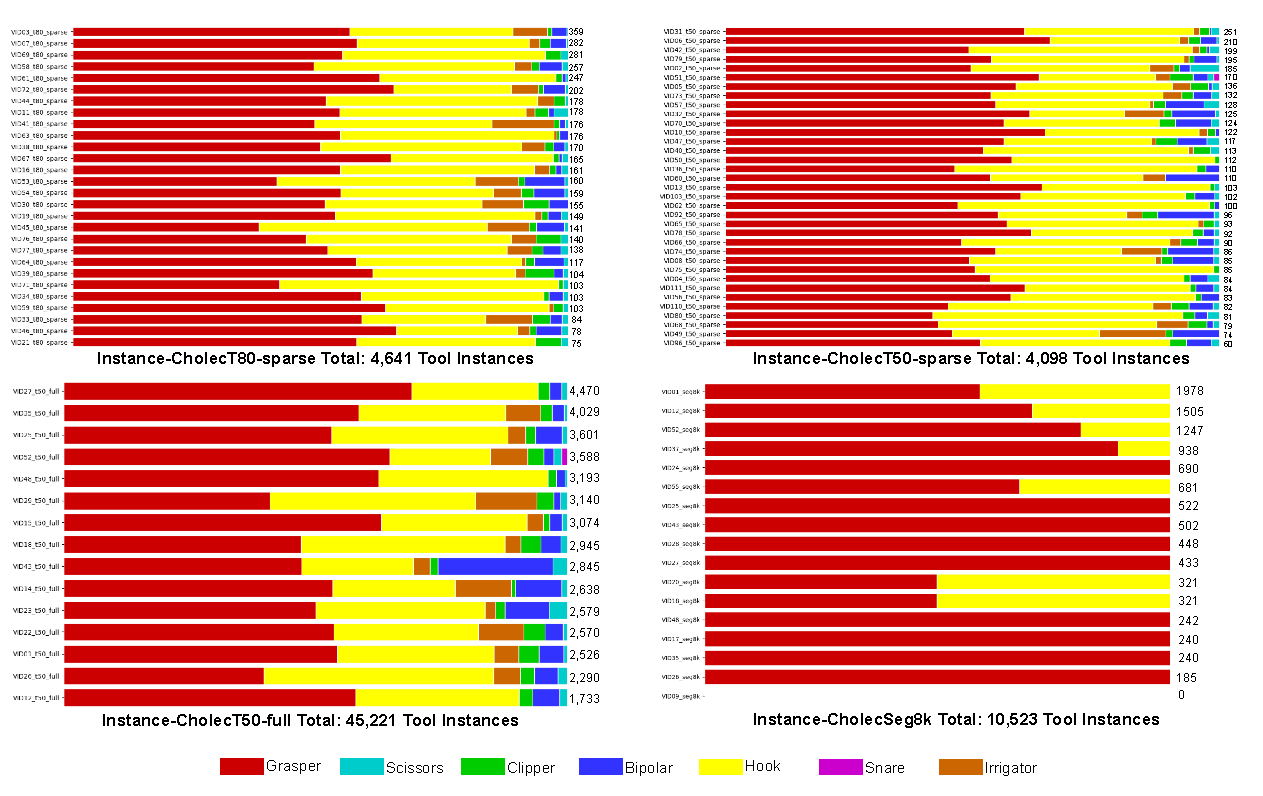
\includegraphics[width=\linewidth]{figs/cholecinstanceseg/charts_sequence_information.pdf}
\caption{Distribution of annotated tool instances across sequences and dataset partitions.}
\label{fig:cholecinstanceseg-sequence-spread}
\end{figure}

\section{Technical Validation}
\label{sec:cholecinstanceseg-validation}

CholecInstanceSeg was validated through baseline model training, label-agreement analysis, and quality-control procedures. Two general-purpose instance segmentation models were trained as baselines: Mask R-CNN \cite{he2017mask} and Mask2Former \cite{cheng2022masked}. These were chosen as broadly applicable reference models rather than specialised surgical-tool architectures, so that future work can compare against a clear baseline.

Performance was evaluated using COCO mean average precision (mAP) and a sequence-aware variant, sequence mAP (smAP). The standard mAP captures class-level segmentation quality, while smAP averages per-sequence performance to better reflect generalisation across surgical scenes. The baseline results are shown in \tabref{tab:cholecinstanceseg-map} and \tabref{tab:cholecinstanceseg-smap}.

\begin{table}[ht]
\centering
\resizebox{\linewidth}{!}{
\begin{tabular}{l|ccccccc|c}
\hline
\textbf{Method} & \textbf{GR} & \textbf{HO} & \textbf{IR} & \textbf{CL} & \textbf{BI} & \textbf{SC} & \textbf{SN} & \textbf{mAP} \\
\hline
Mask R-CNN \cite{he2017mask} & 37.25 & 61.84 & 43.04 & 58.73 & 28.42 & 20.91 & - & 41.70 \\
Mask2Former \cite{cheng2022masked} & 61.10 & 82.16 & 68.38 & 81.30 & 48.02 & 27.89 & - & 61.47 \\
\hline
\end{tabular}}
\caption{Baseline instance segmentation performance on CholecInstanceSeg using mAP. GR: grasper; HO: hook; IR: irrigator; CL: clipper; BI: bipolar; SC: scissors; SN: snare.}
\label{tab:cholecinstanceseg-map}
\end{table}

\begin{table}[ht]
\centering
\resizebox{\linewidth}{!}{
\begin{tabular}{l|ccccccc|c}
\hline
\textbf{Method} & \textbf{GR} & \textbf{HO} & \textbf{IR} & \textbf{CL} & \textbf{BI} & \textbf{SC} & \textbf{SN} & \textbf{smAP} \\
\hline
Mask R-CNN & $41.65\pm12.74$ & $64.06\pm9.20$ & $52.50\pm20.09$ & $64.85\pm16.20$ & $37.62\pm20.74$ & $40.38\pm23.54$ & - & 50.18 \\
Mask2Former & $66.46\pm8.52$ & $88.90\pm7.58$ & $74.51\pm20.35$ & $84.69\pm16.88$ & $65.20\pm25.36$ & $69.76\pm33.20$ & - & 74.92 \\
\hline
\end{tabular}}
\caption{Baseline instance segmentation performance using sequence mAP. The standard deviation indicates variability across sequences.}
\label{tab:cholecinstanceseg-smap}
\end{table}

Mask2Former substantially outperformed Mask R-CNN on both metrics. Hook and clipper achieved high performance, while scissors and bipolar were more challenging, reflecting both lower frequency and visual variability. The smAP results also show that performance can vary considerably across surgical sequences, especially for less common tools.

Inter-annotator agreement was measured on a subset of independently annotated data using panoptic quality \cite{kirillov2019panoptic}. The agreement score was 91.2, indicating strong consistency. Agreement between manual annotations and the semi-automatic annotation pipeline was also measured using panoptic quality, achieving 95.7. These results support the reliability of the annotation process while acknowledging that surgical video annotation remains inherently difficult.

Quality control combined manual review with dataset-specific checks. Frames with more than three tool instances were reviewed, identifying and correcting 26 noisy frames. Cholec80 tool-presence labels were used to cross-check expected tools, identifying 267 frames with errors. Finally, frames with instrument overlaps greater than an IoU threshold of 0.1 were reviewed, leading to corrections in 247 frames.

\section{Limitations and Role in the Thesis}
\label{sec:cholecinstanceseg-limitations}

CholecInstanceSeg has several limitations. It focuses on laparoscopic cholecystectomy, so generalisation to other procedures requires further validation. The annotations are instance-level tool masks rather than full anatomical scene annotations, so they do not directly solve target localisation or tissue understanding. The dataset is also class-imbalanced, reflecting the natural distribution of instruments in cholecystectomy and making rare tools harder to model.

Despite these limitations, CholecInstanceSeg provides the spatial foundation needed for the remainder of this thesis. By distinguishing individual instrument instances, it enables the next step: linking each instrument to the action it performs and the anatomical target it interacts with. \Chapref{chap:triplet-grounding} builds directly on this dataset to move from instrument localisation to grounded surgical interaction understanding.
